\documentclass[a4paper]{article}

\usepackage[utf8]{inputenc}
\usepackage[portuges]{babel}
\usepackage{a4wide}
\usepackage{graphicx}
\usepackage{underscore}
\usepackage{float}
\usepackage{amssymb}
\usepackage{amsmath}


\title{Projeto de Laboratórios de Informática 3\\Grupo 20}
\author{Diogo Miguel Alves Rocha (A79751) \and Gabriela Sá Martins (A81987) \and Ricardo Milhazes Veloso (A81919) \and Ricardo Jorge Silva Ferreira (82568)}
\date{\today}

\begin{document}

\maketitle

\begin{abstract}

O objetivo deste trabalho consistiu em criar um programa que permitisse a extração e análise de dados provenientes da base de dados correspondente ao StackOverFlow. Tendo como objetivo final a resposta a um determinado número de querys , em que o tempo de execução será o mais reduzido possível.
Esta segunda parte do projeto contém o mesmo objetivo da primeira mas desta feita a linguagem de programação usada é Java em vez de C.

\end{abstract}

\tableofcontents

\section{Introdução}
\label{sec:intro}
O trabalho proposto tinha em vista a resolução de 11 interrogações da forma mais eficiente e rápida possível. Para que conseguissemos corresponder a estas medidas criamos quatro estruturas, todas elas HashTables .


\section{Descrição do Problema}

O principal problema era criar uma estrutura capaz de armazenar todos os dados provenientes da base de dados correspondente ao StackOverFlow, de maneira que o acesso a esses mesmos dados fosse o mais rápido possível que por consequência a resposta às interrogações fosse ainda mais rápida, e sem memory leaks.

\section{Concepção da Solução}

Com vista a resolver o problema decidimos criar 4 HashTables, uma com os dados do utilizador,\textbf{id_utilizador},outra com os dados referentes aos posts do tipo pergunta \textbf{id_perguntas},outra com os dados referentes aos posts do tipo resposta \textbf{id_espostas}, e por fim outra com as tags \textbf{id_tags}. Cada uma das anteriores será explicitada numa secção posterior referente às mesmas. 

	\subsection{Porquê da HashTable}

O principal motivo da escolha deste tipo de estrutura de dados foi o tempo de procura de um elemento que no melhor caso vai ser sempre constante e é o tipo de estrutura que apresenta o tempo de procura inferior em relação a outros.

 
\begin{figure}[ht]
\centering
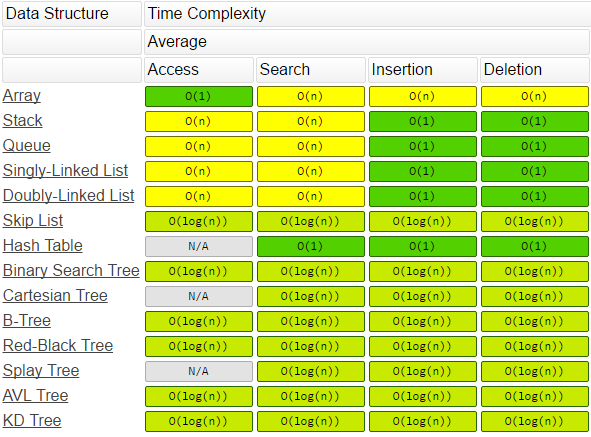
\includegraphics[scale =0.25]{timecomplexity.jpeg}
\caption{timecomplexity}
\label{img:time_complexity}
\end{figure}

\pagebreak

\section{A Estrutura}

\begin{figure}[H]
\centering
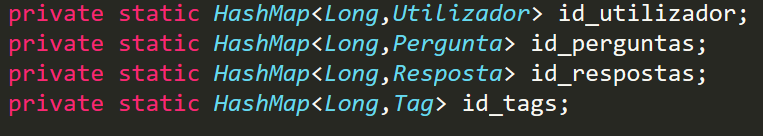
\includegraphics[scale =0.25]{tcd.png}
\caption{Estrutura}
\label{img:tcd}
\end{figure}

	\subsection{id_utilizador}
	A estrutura contém informações relativas ao \textbf{utilizador}, e apresenta 7 parâmetros diferentes:

	\begin{description}
		\item[id_u] -ID do utilizador;
		\item[name] -Nome do utilizador;
		\item[shortb] -Short bio do utilizador;
		\item[totalposts] -Número total de posts;
		\item[reputacao] -Reputação do utilizador;
		\item[votes] -Número de votes do utilizador;
	\end{description}
	

	\begin{figure}[H]
	\centering
	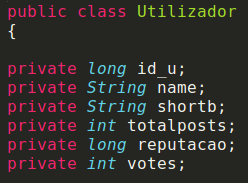
\includegraphics[scale =0.25]{utilizador.png}
	\caption{id_utilizador}
	\label{img:id_utilizador}
	\end{figure}

	\subsection{id_perguntas}
	A estrutura contém informações relativas às \textbf{Perguntas}, e apresenta 7 parâmetros diferentes:

	\begin{description}
		\item[id_post] -ID da pergunta;
		\item[id_autor] -ID do autor da pergunta;
		\item[title] -Título da pergunta;
		\item[tags] -Tag da pergunta;
		\item[reputacao] -Reputação do utilizador;
		\item[n_resp] -Número de respostas àquela pergunta;
		\item[d] -Data da pergunta;
	\end{description}


	\begin{figure}[H]
	\centering
	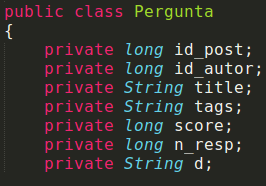
\includegraphics[scale =0.25]{perguntas.png}
	\caption{id_perguntas}
	\label{img:id_perguntas}
	\end{figure}

	\subsection{id_respostas}
	A estrutura contém informações relativas às \textbf{Respostas}, e apresenta 6 parâmetros diferentes:

	\begin{description}
		\item[id_post] -ID da Resposta;
		\item[id_perg] -ID da pergunta correspondente à resposta;
		\item[id_autor] -ID do autor da resposta;
		\item[score] -Score da resposta;
		\item[n_coments] -Número de comentários aquela resposta;
		\item[d] -Data da Resposta;

	\end{description}


	

	\begin{figure}[H]
	\centering
	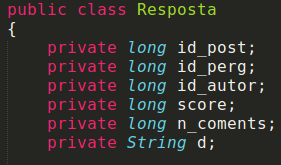
\includegraphics[scale =0.25]{respostas.png}
	\caption{id_respostas}
	\label{img:id_respostas}
	\end{figure}

	\subsection{id_tags}
	A estrutura contém informações relativas às \textbf{Tags}, e apresenta 3 parâmetros diferentes:

	\begin{description}
		\item[id_tag] -ID da tag;
		\item[tag] -Tag;
		\item[count] -Conta o número de vezes que uma Tag é utilizada num intervalo de tempo;
	\end{description}	


	\begin{figure}[H]
	\centering
	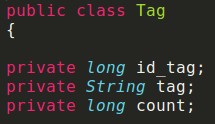
\includegraphics[scale =0.25]{tags.png}
	\caption{id_tags}
	\label{img:id_tags}
	\end{figure}

	
\pagebreak
\section {Extração de Informação}

	\subsection{Pergunta 1}
	Na pergunta 1 temos de retornar um par com o titulo do post correspondente ao id recebido, e com o nome do utilizador a que esse post pertence. 
	Para isso acedemos à \textbf{id_perguntas} retiramos o titulo e o nome do autor correspondente ao id recebido e retornamos um par com os respetivos. 

	\subsection{Pergunta 2}
		Nesta pergunta queremos saber o Top N utilizadores com maior número de posts e para isso consultamos a variável totalposts, através do método que implementamos na classe Utilizador \textbf{getTotalposts()},após utilizarmos um \textbf{ArrayList} infoPost que guarda toda a informação existente na \textbf{id_utilizador}. De seguida ordenamos esse ArrayList pelo número total de posts. E no fim retornamos um List com os \textbf{id_u} ordenados.

	\subsection{Pergunta 3}
		Nesta pergunta queremos obter o número total de posts num determinado periodo de tempo mas com perguntas e respostas em separado. Para isso percorremos a \textbf{id_perguntas}  e a \textbf{id_respostas}, e utilizando o método \textbf{compareTo()}, retiramos todas as perguntas e respostas, respetivamente que se encontram entre as datas recebidas. No fim retornamos um par com essas perguntas e respostas.

	\subsection{Pergunta 4}
		Nesta pergunta queremos obter o número total de perguntas contendo uma determinada tag num determinado periodo de tempo, e retornar essas perguntas por cronologia inversa.
		Para isso percorremos a \textbf{id_perguntas} e utilizando o método \textbf{compareTo}e o método \textbf{contains} ,retiramos todas as perguntas que se encontram entre as datas recebidas e que contém uma tag igual à recebida, e adicionamos estas perguntas a um \textbf{ArrayList} TagsData. Em seguida ordenamos este ArrayList por data (da mais recente para a mais antiga) utilizando novamente o método \textbf{compareTo()}. Por fim adicionamos numa List todos os id_post que contêm aquela tag, retornado essa List.

	\subsection{Pergunta 5}
		Nesta pergunta queremos devolver a informação do
		perfil do utilizador (short bio) e os IDs dos seus 10 últimos posts (perguntas ou respostas),ordenados por cronologia inversa. Para isso utilizamos um \textbf{Utilizador} u para guardar a informação de um utilizador corresponde ao id recebido, depois acedemos a esse Utilizador para retirar a shorbio.
		Em seguida criamos um \textbf{ArrayList}ultimasPerg e um \textbf{ArrayList} ultimasResp e utilizamos o método \textbf{Long.compare} em ambos os casos para comparar se o id recebido corresponde a uma pergunta ou a uma resposta  se algum dos casos se verificar adiciona uma pergunta na \textbf{ultimasPerg} ou uma resposta na \textbf{ultimasResp}.
		Em seguida criamos uma \textbf{LinkedHashMap} result e adicionamos o id_post e a data retirados do ultimasPerg e do ultimasResp. Depois ordenamos esse LinkedHashmap pela data. Por fim criamos um List(res) que recebe todas as keys da LinkedHashmap já ordenada e depois adicionamos noutro List(f) as 10 primeiras keys. E retornamos um par com a shortbio e com a List f.

	\subsection{Pergunta 6}
		Nesta pergunta queremos saber, num intervalo de tempo arbitrario, quais as N respostas com mais votos, devolvendo uma lista com  a variável id_post. Para isso criamos um \textbf{ArrayList}.Em seguida percorremos essa a id_respostas e utilizando o método \textbf{compareTo} adicionamos à resp_Data todas as respostas que se encontrem entre a data recebida. Em seguida ordenamos a resp_data através do Score(por ordem decrescente) , e criamos um \textbf{List} res um N id_post . Por fim retorna esse mesmo res.
	\subsection{Pergunta 7}
		Nesta pergunta queremos obter os IDs das N perguntas com mais respostas, por ordem decrescentem num determinado intervalo de tempo. Para isso consultamos a variável n_resp, através do método que implementamos na classe Pergunta \textbf{getN_resp()}, após utilizarmos um \textbf{ArrayList<Pergunta>} que guarda toda a informação existente na \textbf{id_perguntas} dentro das datas fornecidas. De seguida, ordenamos esse ArrayList de acordo com o número de respostas (por ordem decrescente) e por fim, retornamos um List com os N \textbf{id_post} das perguntas com mais respostas ordenado.
	\subsection{Pergunta 8}
		Nesta pergunta queremos obter os IDs das N perguntas cujos títulos contém uma palavra específica, ordenados por cronologia inversa. Para isso percorremos a \textbf{id_perguntas} e utilizando \textbf{compareTo} e o método \textbf{contains}. Guardamos todas as perguntas cujos títulos continham a palavra fornecida num \textbf{ArrayList<Pergunta>}, e depois ordenamos o mesmom de acordo com a data da pergunta. Por fim, retornamos um List com os N \textbf{id_post} das perguntas que continham no título a palavra dada, ordenados por cronologia inversa.

	\subsection{Pergunta 9}
		Nesta pergunta recebendo o ID de dois utilizadores devolver as últimas N perguntas que em que participaram esses dois utilizadores.
		Para isso criamos um \textbf{ArrayList} resps e um \textbf{ArrayList} perg final e guardamos todas as respostas da id_respostas na resps. Em seguida usamos o método \textbf{Long.compare} para comparar o id do autor com o id1 recebido e adicionamos em p1 a pergunta que contenha aquele id. Após isto se o id2 for igual o id_autor adiciona p1 na pergsFinal. Em seguida utiliza o mesmo método mas para a resposta. Depois ordena o pergsFinal por data , cria uma List res e adiciona N id_post a essa lista res. Por fim retorna essa mesma lista.
	\subsection{Pergunta 10}
		Nesta pergunta queremos obter a melhor resposta a uma pergunta específica, utilizando a função de média (Score da resposta x 0.45) + (Reputação do utilizador x 0.25) + (número de Votos recebidos pela resposta x 0.2) + (número de comentários recebidos pela resposta x 0.1). Para isso percorremos a \textbf{id_respostas} guardando num \textbf{ArrayList<Resposta>} as respostas correspondentes à pergunta cujo ID foi dado, através do método \textbf{getID_perg()}. Em seguida, é percorrida a \textbf{id_utilizador} e são guardados os utilizadores a quem corresponde a resposta. Depois acedemos às variáveis score, n_coments e reputacao através dos métodos \textbf{getScore()}, \textbf{getN_coments()}, \textbf{getReputacao()}, respetivamente, implementadas na classe Utilizador. De seguida são efetuados os cálculos de acordo com a fórmula anteriormente referida e os valores resultantes vão sendo comparados até se obter a melhor resposta e esta ser retornada.
	\subsection{Pergunta 11}
		Infelizmente não conseguimos um resultado positivo nesta pergunta.

\pagebreak
\section{LI3 em java vs LI3 em C}

No projeto de LI3 em java chegamos á conclusao que, comparativamente com este em C, este apresenta beneficios ao nivel do tratamento de excecçoes , uso de memória, compilação do código e a portabilidade.
Tratamento de exceçoes 
A linguagem java apresenta beneficios ao nivel do tratamento de exceçoes pois esta admite recursos para o tratamento das mesmas

Uso de memoria 
Na linguagem java o uso de memoria é mais superficial comparado com a linguagem C. Em C foi necessario o uso de apontadores e definicao da capacacidade dos arrays etc. Enquanto que em java nao é necessaria essa preocupacao pois o proprio java aloca o espaço necessario para o carregamento da estrutura que etsmaos a definir
O que torna a programacao em java mais facil mas tambem menos controlavel

Utilizacao de librarias 
Em Java existem librarias em que a ordenacao, insercao em hashtables, tratamento de exceçoes etc ja estao implementadas e bem implementadas. Enquanto que em C existem menos e a maioria tem de ser escrita o que proporciona uma maior probablidade de erros e bugs.
		
\section {Resultados}

\begin{figure}[H]
	\centering
	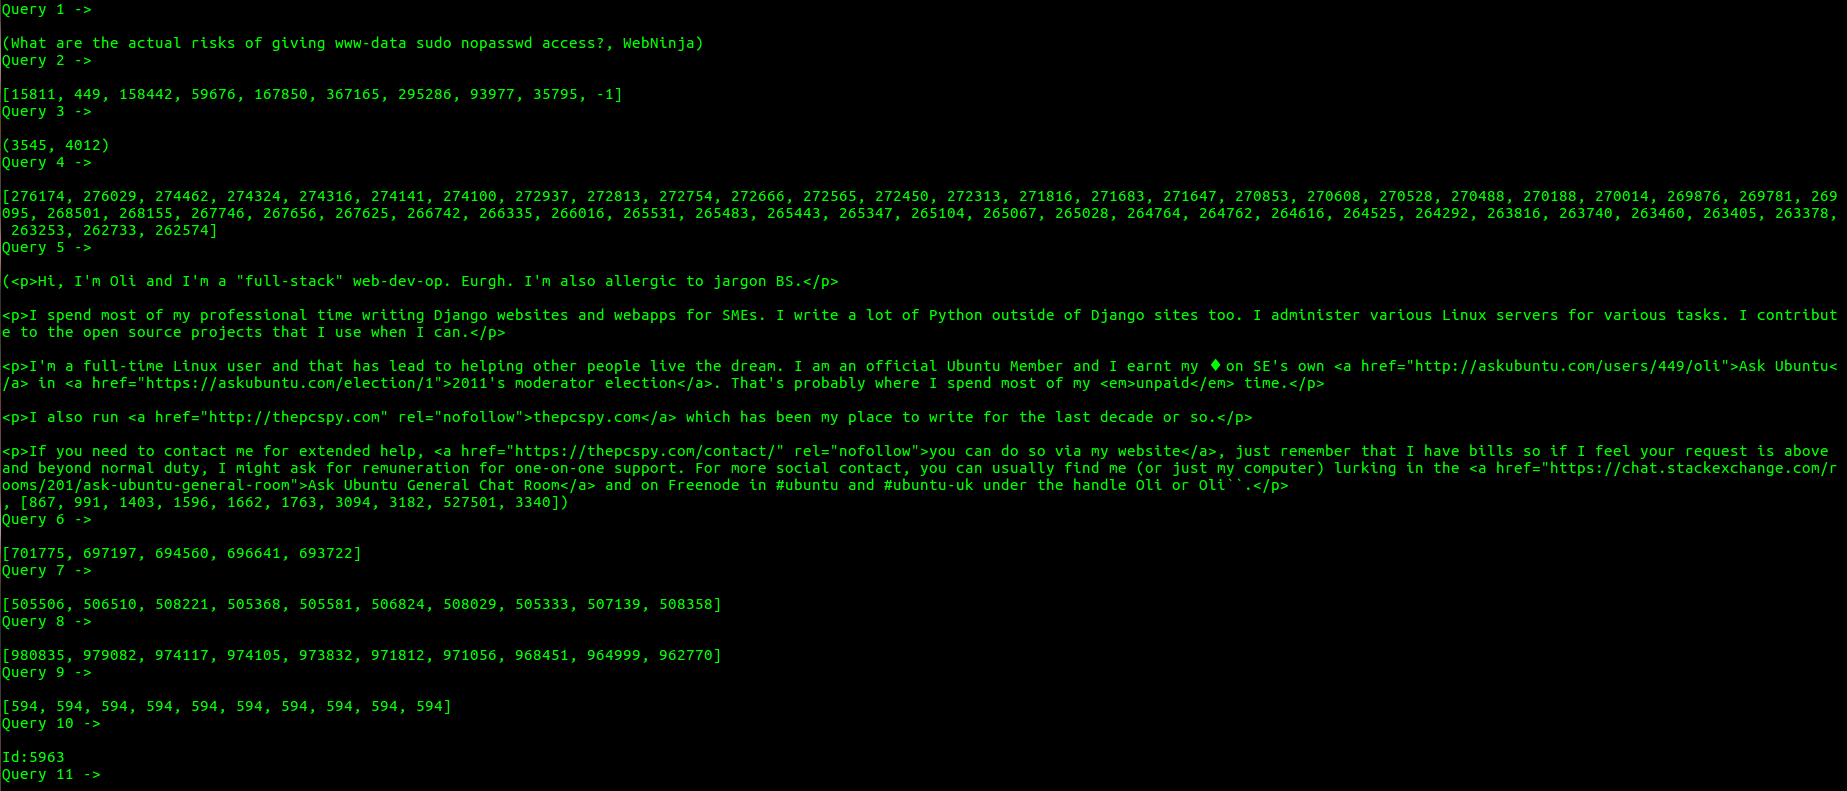
\includegraphics[scale =0.23]{resultados.png}
	\caption{Resultados}
	\label{img:Resultados}
	\end{figure}

\section {Teste de Tempo}

\begin{figure}[H]
	\centering
	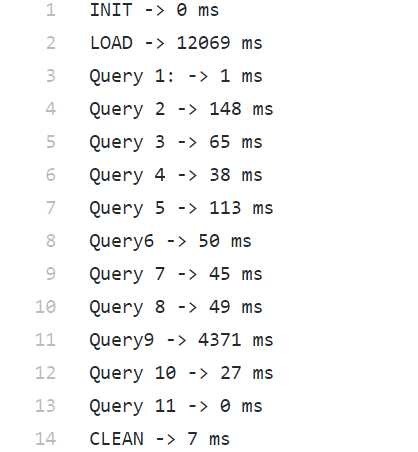
\includegraphics[scale =0.20]{tempo.png}
	\caption{tempo}
	\label{img:tempo}
	\end{figure}


\section{Conclusão}

Em suma quase todos os objetivos propostos foram atingidos, apenas os resultados pretendidos não foram atingidos na query 5 em que o return não é o correto e na query 11 que não conseguimos criar uma maneira de a resolver. Toda a extração de informação proveniente da base de dados do site \textbf{StackOverflow} e análise da mesma é feita de uma maneira eficiente, com um tempo de execução bastante aceitável e sem qualquer perda de informação. Esta segunda fase do projeto foi bastante útil para desenvolver competencias na linguagem de programação java bem como aprender a utilizar a ferramenta \textbf{Maven}. 
Por tudo isto acreditamos que a segunda fase do projeto foi concluida com sucesso.


\end{document}